\section{Evidence}
\label{sec:experiments}

The validation addresses the tool's two roles, holding during a shift and guiding a turn, and then their composition. The available hardware trials test the turn; shifts, complete sequences, and the quantitative predictions of Sections~\ref{sec:method}--\ref{sec:tworod} are tested in simulation.

\subsection{Turns on hardware and in simulation}
\label{sec:exp_turn}

The turn was run on a first-generation Kinova Jaco and in MuJoCo \cite{todorov2012mujoco} for four configurations of one elongated rectangle, with five hardware trials and one simulation run per configuration. A single bearing-mounted rod was installed once and calibrated. For each request, the rod centre was placed at $\mathbf P_i+R\mathbf n_i$, the vertex and adjacent edge normal with the largest lever arm in the requested direction; this is a vertex contact covered by the orbit argument of Section~\ref{sec:orbit}. The grasp point differed between configurations. A camera measured the initial and final orientations, with a marker on the object resolving the rectangle's symmetry, and a force/torque sensor attached to the rod detected first contact and its direction. The approach was planned as in Section~\ref{sec:approach}. The arm then followed \eqref{eq:rod_path} with fixed wrist orientation and no feedback (\figref{fig:experiment_setup}).

\begin{figure}[htbp]
\centering
% Figure7.jpg and Figure8.jpg are JPEG copies (quality 90) of the hardware
% photographs, Figure7 resized to 1200 px wide; the originals are kept out of
% the repository (see README). Nothing else is edited. Native clipping only
% enlarges the contact region in the three original bottom-row hardware frames.
\begin{tikzpicture}[paperfigure]
  \path[use as bounding box] (0,0) rectangle (15.3,5.05);
  \node[paneltitle] at (0,4.85) {(a) Experimental setup};
  \node[anchor=south west,inner sep=0] at (0,0)
    {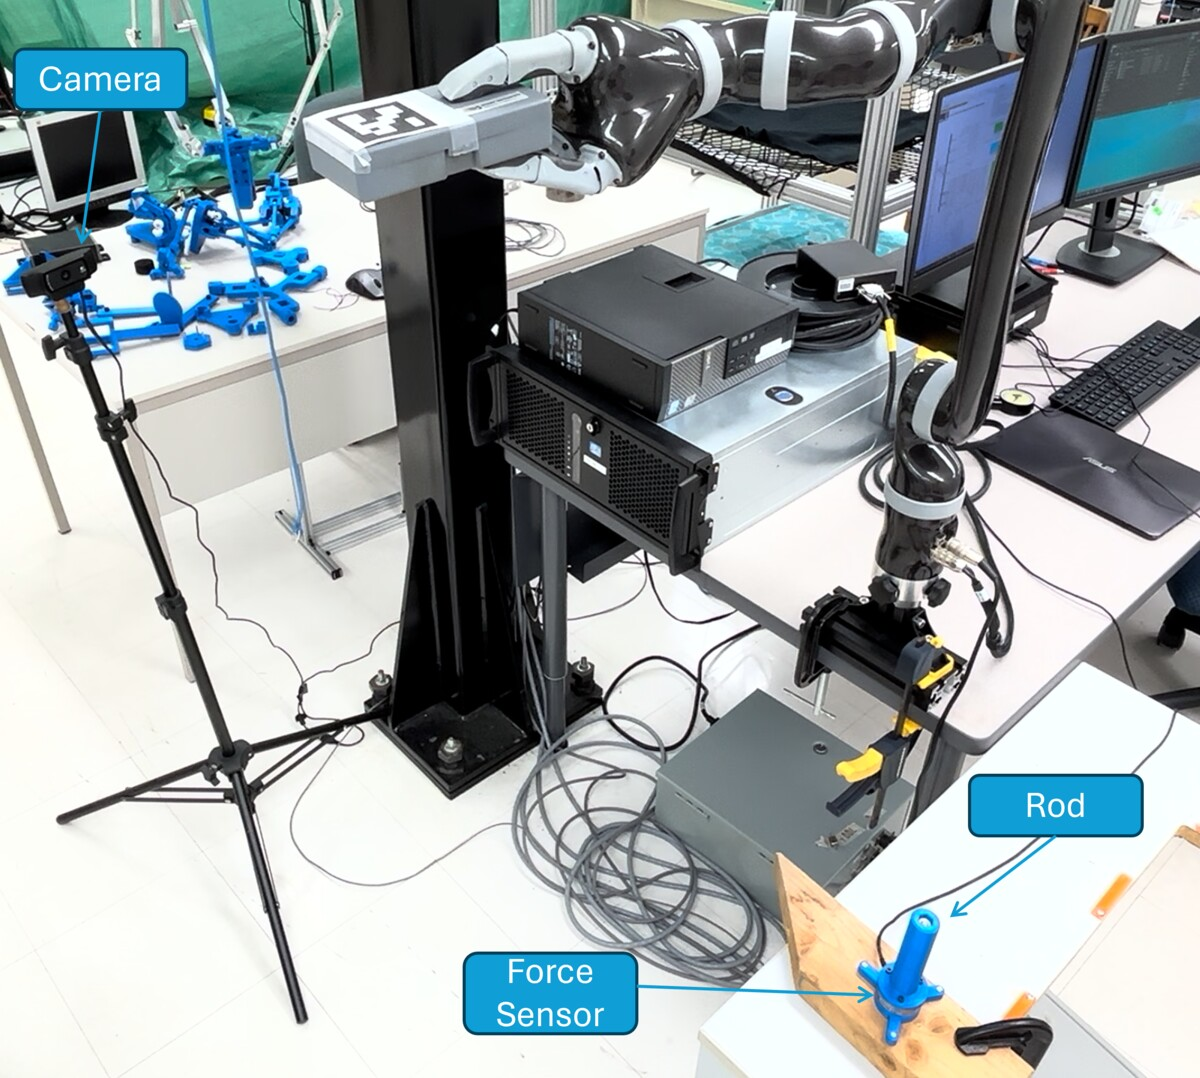
\includegraphics[width=5.1cm]{Figure7.jpg}};
  \node[paneltitle] at (6.0,4.85) {(b) MuJoCo sequence};
  \node[anchor=south west,inner sep=0] at (6.0,.95)
    {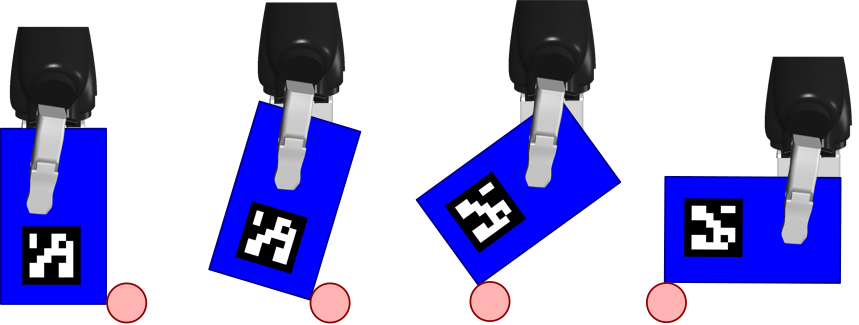
\includegraphics[width=8.4cm]{Figure6.png}};
  \foreach \x/\stage in {6.84/1,8.87/2,11.18/3,13.59/4} {
    \draw[motion,line width=1.1pt] (\x,3.95) -- ++(.385,0);
    \node[anchor=north] at (\x+.15,.85) {Stage \stage};
  }
  \node[anchor=west] at (6.0,.1) {Parallel arrows: fixed wrist orientation};
\end{tikzpicture}

\vspace{2mm}
\begin{tikzpicture}[paperfigure]
  \path[use as bounding box] (0,-.55) rectangle (15.3,5.1);
  \node[paneltitle] at (0,4.92) {(c) Hardware contact region};
  % Figure8.jpg is 3033 by 1819 pixels. Its three bottom frames
  % have equal widths. Identical lower-right regions are shown at the same scale.
  \foreach \x/\sx/\stage in {
    0/-5.5/{Approach / contact},
    5.3/-15.61/{Intermediate},
    10.6/-25.72/{Final}}
  {
    \begin{scope}[shift={(\x,0)}]
      \clip (0,0) rectangle (4.61,4.595);
      \node[anchor=south west,inner sep=0] at (\sx,0)
        {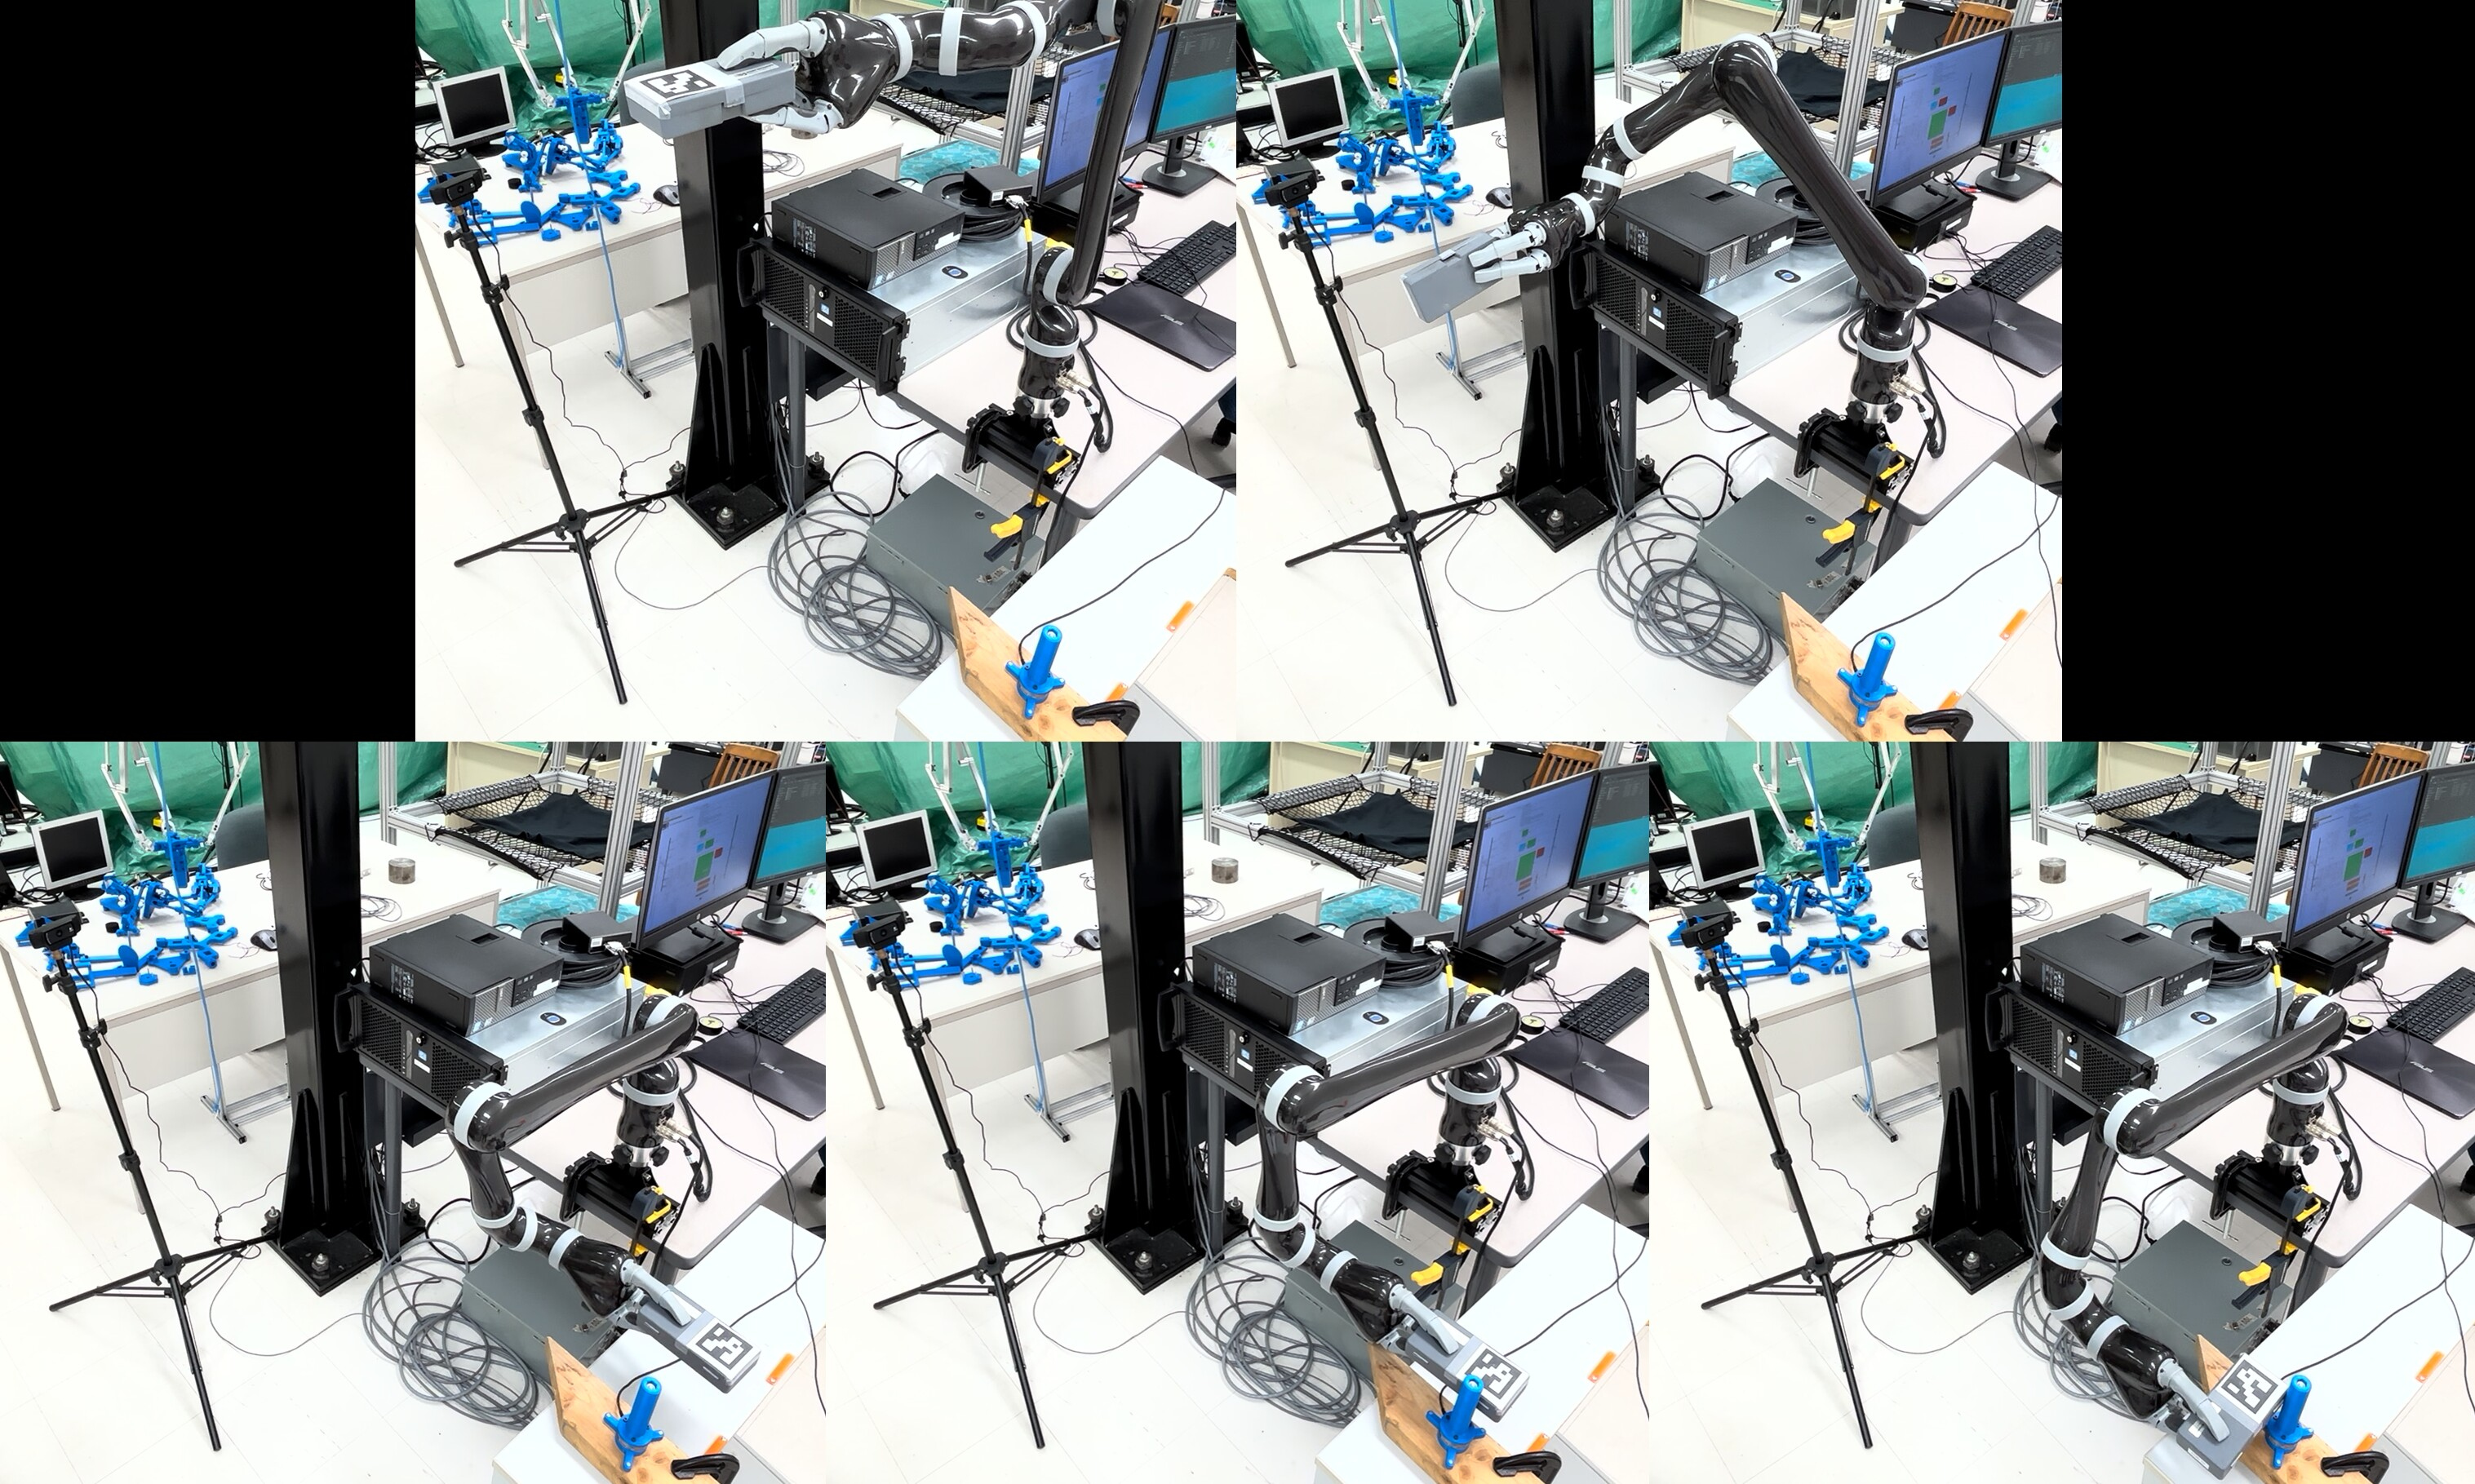
\includegraphics[width=30.33cm]{Figure8.jpg}};
    \end{scope}
    \node[anchor=north,text width=4.61cm,align=center] at (\x+2.305,-.1) {\stage};
  }
\end{tikzpicture}
\caption{Original setup and MuJoCo sequence, with three enlarged hardware contact-region crops in their original order. Stage labels carry no measured timestamps or angles.}
\label{fig:experiment_setup}
\end{figure}


\begin{table}[htbp]
    \centering
    \renewcommand{\arraystretch}{1.1}
    \begin{tabular}{ccc}
        \hline
        Initial $\rightarrow$ target ($^{\circ}$) & Simulation error ($^{\circ}$) & Hardware MAE ($^{\circ}$, $n=5$) \\
        \hline
        $0\rightarrow90$ & 0.2 & 3.6 \\
        $90\rightarrow180$ & 0.1 & 4.1 \\
        $-90\rightarrow0$ & 0.3 & 7.5 \\
        $180\rightarrow0$ & 0.2 & 4.9 \\
        \hline
    \end{tabular}
    \caption{Absolute final-angle errors of the turn: one simulation run and five hardware trials per configuration.}
    \label{tab:results}
\end{table}

The hardware mean absolute errors were $3.6^{\circ}$--$7.5^{\circ}$ (\tabref{tab:results}). Only these means were retained; signed errors, trial spread, pad dimensions, and grasp drift are unavailable. The trials therefore demonstrate the turn primitive, including its vertex-contact case, but cannot test the sign or magnitude of the under-rotation predicted by Proposition~\ref{prop:slip}.

\subsection{Shifts and complete sequences in simulation}
\label{sec:exp_tworod}

\paragraph{Configuration and predictions.}
The simulations use an $80\times30$ mm rectangular plate grasped at its centre, rods of radius $R=5$ mm, and the request $\Delta=\pi/2$, $\mathbf d=(5,20)$ mm. Then $\mathbf d_0=(20,-5)$ mm, the trailing vertex is $(-40,15)$ mm, and the weights are $\alpha_a\simeq0.24$ for the top edge and $\alpha_b\simeq0.97$ for the left edge. The meeting point $\mathbf x=(-36,9)$ mm ($\lambda\simeq37.1$ mm) gives rod centres $(-36,20)$ and $(-45,9)$ mm, spacing $D\simeq14.2$ mm, and $K_{\mathrm{sh}}\simeq11.4$ mm/rad. After the shift, the top rod has lever arm $\ell=16.0$ mm and drives the quarter turn, while the left rod's lever arm is $-4$ mm and its contact separates. Sections~\ref{sec:method} and~\ref{sec:turn} then predict the following. A placement error $e$ makes the plate tilt toward $e/K_{\mathrm{sh}}$, that is $5.0^{\circ}$ per millimetre, but by \eqref{eq:relax_end} a shift of $\|\mathbf d_0\|=20.6$ mm from an untilted start reaches only $32\%$ of it, $1.59^{\circ}$ per millimetre; for the stiffer placement $\lambda=30$ mm ($K_{\mathrm{sh}}=18.5$ mm/rad), it reaches $74\%$, $2.28^{\circ}$ per millimetre. A pad with limit-surface length $\rho$ (in millimetres) makes the turn under-rotate by $0.35\rho^2$ degrees, with a grasp drift of $0.098\rho^2$ mm toward the top edge.

\paragraph{Model.}
The simulations use MuJoCo 3.14 \cite{todorov2012mujoco}. The plate is 5 mm thick, has a mass of 0.2 kg, and touches only the pads and the rods, with gravity off. The gripper translates on two prescribed slide joints with its orientation locked, and two spherical pads of radius 1 mm pinch the plate with a constant force of 5 N each. Each pad is a single elliptic-cone contact with torsional friction, which gives the ellipsoidal limit surface of Section~\ref{sec:slip} with $\rho$ equal to the ratio of torsional to sliding friction; $\rho=2$ mm unless varied, which corresponds to a uniformly loaded disk pad of radius 3 mm. The rods have radius 5 mm and spin on undamped hinges. They are frictionless except in the comparison of free and fixed rods below: with rod friction, the solver transmitted a spurious tangential force of about 0.2--0.3 N through a free rod, which made runs with small rod loads depend on the time step, whereas by Section~\ref{sec:freerod} a free rod's wrench does not depend on its friction, which that comparison checks. Shifts run at 5 mm/s and turns at $10^{\circ}$/s with a time step of 1 ms. Of the 367 runs, 17 repeat a case at half or quarter time step and 11 at half speed; these repeats changed final angles by at most $0.04^{\circ}$. Holding the plate still against the rods for the 9 s of a turn moved it by $0.02^{\circ}$ and 0.03 mm, which bounds the solver's creep.

\paragraph{Shift.}
With the rods at the nominal placement, we offset the initial grasp across the drag line so that $e\in\{0,\pm0.5,\pm1\}$ mm and ran the shift alone. The endpoint tilt had the sign of $e$ and was linear in it, with slopes of $1.589^{\circ}$ and $2.267^{\circ}$ per millimetre for $\lambda=37.1$ and 30 mm (residuals below $0.01^{\circ}$), against $1.59^{\circ}$ and $2.28^{\circ}$ from \eqref{eq:relax_end} and asymptotes of $5.03^{\circ}$ and $3.10^{\circ}$, and along the shift it followed the solution of \eqref{eq:relax} to within $0.02^{\circ}$ (\figref{fig:sim_shift}). Halving the shift speed changed the endpoints by less than $0.01^{\circ}$, so the tilt is set by the distance travelled rather than by time, and a 3 s hold after the shift changed them by less than $0.04^{\circ}$. For a shift pushed straight into the top edge, with the rods offset by 0.5 mm along it, a single rod let the plate turn by $2.76^{\circ}$ and move by 0.48 mm over the 10 mm shift, whereas two rods straddling the grasp line held it within $0.003^{\circ}$ and 0.02 mm, as Section~\ref{sec:minimal} predicts.

\begin{figure}[htbp]
\centering
% Written by python -m simulation figures from results/simulation.json; do not edit by hand.
\begin{tikzpicture}[paperfigure]
\path[use as bounding box] (0,-0.6) rectangle (15.6,6.0);
\draw[black!12,line width=.3pt] (1.300,1.657) -- (7.100,1.657);
\draw[black!12,line width=.3pt] (1.300,2.479) -- (7.100,2.479);
\draw[black!12,line width=.3pt] (1.300,3.300) -- (7.100,3.300);
\draw[black!12,line width=.3pt] (1.300,4.121) -- (7.100,4.121);
\draw[black!12,line width=.3pt] (1.300,4.943) -- (7.100,4.943);
\draw[black!35,line width=.4pt] (1.300,3.300) -- (7.100,3.300);
\draw[black!35,line width=.4pt] (4.200,1.000) -- (4.200,5.600);
\draw[black!60,line width=.4pt] (1.300,1.000) rectangle (7.100,5.600);
\draw[black!60,line width=.4pt] (1.678,1.000) -- ++(0,.08) node[below=3pt,black!80] {$-1$};
\draw[black!60,line width=.4pt] (2.939,1.000) -- ++(0,.08) node[below=3pt,black!80] {$-0.5$};
\draw[black!60,line width=.4pt] (4.200,1.000) -- ++(0,.08) node[below=3pt,black!80] {$0$};
\draw[black!60,line width=.4pt] (5.461,1.000) -- ++(0,.08) node[below=3pt,black!80] {$0.5$};
\draw[black!60,line width=.4pt] (6.722,1.000) -- ++(0,.08) node[below=3pt,black!80] {$1$};
\draw[black!60,line width=.4pt] (1.300,1.657) -- ++(.08,0) node[left=3pt,black!80] {$-4$};
\draw[black!60,line width=.4pt] (1.300,2.479) -- ++(.08,0) node[left=3pt,black!80] {$-2$};
\draw[black!60,line width=.4pt] (1.300,3.300) -- ++(.08,0) node[left=3pt,black!80] {$0$};
\draw[black!60,line width=.4pt] (1.300,4.121) -- ++(.08,0) node[left=3pt,black!80] {$2$};
\draw[black!60,line width=.4pt] (1.300,4.943) -- ++(.08,0) node[left=3pt,black!80] {$4$};
\node[below=14pt] at (4.200,1.000) {offset $e$ (mm)};
\node[rotate=90,above=18pt] at (1.300,3.300) {endpoint tilt ($^{\circ}$)};
\draw[objectblue,densely dashed,line width=.6pt] (1.426,1.029) -- (6.974,5.571);
\draw[objectblue,line width=.8pt] (1.426,2.580) -- (6.974,4.020);
\filldraw[fill=objectblue,draw=white,line width=.4pt] (6.722,3.955) circle[radius=2.1pt];
\filldraw[fill=objectblue,draw=white,line width=.4pt] (5.461,3.625) circle[radius=2.1pt];
\filldraw[fill=objectblue,draw=white,line width=.4pt] (4.200,3.297) circle[radius=2.1pt];
\filldraw[fill=objectblue,draw=white,line width=.4pt] (2.939,2.972) circle[radius=2.1pt];
\filldraw[fill=objectblue,draw=white,line width=.4pt] (1.678,2.650) circle[radius=2.1pt];
\draw[forceorange,densely dashed,line width=.6pt] (1.426,1.901) -- (6.974,4.699);
\draw[forceorange,line width=.8pt] (1.426,2.271) -- (6.974,4.329);
\filldraw[fill=forceorange,draw=white,line width=.4pt] (6.722,4.236) ++(-1.9pt,-1.9pt) rectangle ++(3.8pt,3.8pt);
\filldraw[fill=forceorange,draw=white,line width=.4pt] (5.461,3.766) ++(-1.9pt,-1.9pt) rectangle ++(3.8pt,3.8pt);
\filldraw[fill=forceorange,draw=white,line width=.4pt] (4.200,3.299) ++(-1.9pt,-1.9pt) rectangle ++(3.8pt,3.8pt);
\filldraw[fill=forceorange,draw=white,line width=.4pt] (2.939,2.835) ++(-1.9pt,-1.9pt) rectangle ++(3.8pt,3.8pt);
\filldraw[fill=forceorange,draw=white,line width=.4pt] (1.678,2.375) ++(-1.9pt,-1.9pt) rectangle ++(3.8pt,3.8pt);
\node[anchor=south west,font=\small\bfseries] at (1.300,5.600) {(a)};
\filldraw[fill=objectblue,draw=white,line width=.4pt] (1.678,5.189) circle[radius=2.1pt];
\node[anchor=west,font=\scriptsize] at (1.880,5.189) {$\lambda=37.1$ mm};
\filldraw[fill=forceorange,draw=white,line width=.4pt] (1.678,4.820) ++(-1.9pt,-1.9pt) rectangle ++(3.8pt,3.8pt);
\node[anchor=west,font=\scriptsize] at (1.880,4.820) {$\lambda=30$ mm};
\draw[black!12,line width=.3pt] (9.200,1.000) -- (15.000,1.000);
\draw[black!12,line width=.3pt] (9.200,1.767) -- (15.000,1.767);
\draw[black!12,line width=.3pt] (9.200,2.533) -- (15.000,2.533);
\draw[black!12,line width=.3pt] (9.200,3.300) -- (15.000,3.300);
\draw[black!12,line width=.3pt] (9.200,4.067) -- (15.000,4.067);
\draw[black!12,line width=.3pt] (9.200,4.833) -- (15.000,4.833);
\draw[black!60,line width=.4pt] (9.200,1.000) rectangle (15.000,5.600);
\draw[black!60,line width=.4pt] (9.200,1.000) -- ++(0,.08) node[below=3pt,black!80] {$0$};
\draw[black!60,line width=.4pt] (10.581,1.000) -- ++(0,.08) node[below=3pt,black!80] {$5$};
\draw[black!60,line width=.4pt] (11.962,1.000) -- ++(0,.08) node[below=3pt,black!80] {$10$};
\draw[black!60,line width=.4pt] (13.343,1.000) -- ++(0,.08) node[below=3pt,black!80] {$15$};
\draw[black!60,line width=.4pt] (14.724,1.000) -- ++(0,.08) node[below=3pt,black!80] {$20$};
\draw[black!60,line width=.4pt] (9.200,1.000) -- ++(.08,0) node[left=3pt,black!80] {$0$};
\draw[black!60,line width=.4pt] (9.200,1.767) -- ++(.08,0) node[left=3pt,black!80] {$1$};
\draw[black!60,line width=.4pt] (9.200,2.533) -- ++(.08,0) node[left=3pt,black!80] {$2$};
\draw[black!60,line width=.4pt] (9.200,3.300) -- ++(.08,0) node[left=3pt,black!80] {$3$};
\draw[black!60,line width=.4pt] (9.200,4.067) -- ++(.08,0) node[left=3pt,black!80] {$4$};
\draw[black!60,line width=.4pt] (9.200,4.833) -- ++(.08,0) node[left=3pt,black!80] {$5$};
\node[below=14pt] at (12.100,1.000) {grasp travel $s$ (mm)};
\node[rotate=90,above=18pt] at (9.200,3.300) {tilt ($^{\circ}$)};
\draw[objectblue,densely dashed,line width=.6pt] (9.200,4.854) -- (15.000,4.854);
\draw[objectblue,line width=.8pt] (9.200,1.000) -- (9.314,1.013) -- (9.428,1.027) -- (9.542,1.041) -- (9.657,1.055) -- (9.771,1.069) -- (9.885,1.084) -- (9.999,1.099) -- (10.113,1.114) -- (10.227,1.129) -- (10.342,1.145) -- (10.456,1.161) -- (10.570,1.178) -- (10.684,1.195) -- (10.798,1.212) -- (10.912,1.230) -- (11.027,1.248) -- (11.141,1.266) -- (11.255,1.285) -- (11.369,1.304) -- (11.483,1.324) -- (11.597,1.344) -- (11.712,1.364) -- (11.826,1.386) -- (11.940,1.407) -- (12.054,1.429) -- (12.168,1.452) -- (12.282,1.475) -- (12.397,1.499) -- (12.511,1.523) -- (12.625,1.548) -- (12.739,1.574) -- (12.853,1.600) -- (12.967,1.628) -- (13.081,1.655) -- (13.196,1.684) -- (13.310,1.713) -- (13.424,1.743) -- (13.538,1.774) -- (13.652,1.806) -- (13.766,1.839) -- (13.881,1.873) -- (13.995,1.907) -- (14.109,1.943) -- (14.223,1.980) -- (14.337,2.018) -- (14.451,2.057) -- (14.566,2.098) -- (14.680,2.139) -- (14.794,2.182);
\filldraw[fill=objectblue,draw=white,line width=.4pt] (9.476,1.026) circle[radius=2.1pt];
\filldraw[fill=objectblue,draw=white,line width=.4pt] (10.029,1.096) circle[radius=2.1pt];
\filldraw[fill=objectblue,draw=white,line width=.4pt] (10.581,1.173) circle[radius=2.1pt];
\filldraw[fill=objectblue,draw=white,line width=.4pt] (11.133,1.258) circle[radius=2.1pt];
\filldraw[fill=objectblue,draw=white,line width=.4pt] (11.686,1.354) circle[radius=2.1pt];
\filldraw[fill=objectblue,draw=white,line width=.4pt] (12.238,1.460) circle[radius=2.1pt];
\filldraw[fill=objectblue,draw=white,line width=.4pt] (12.791,1.581) circle[radius=2.1pt];
\filldraw[fill=objectblue,draw=white,line width=.4pt] (13.343,1.718) circle[radius=2.1pt];
\filldraw[fill=objectblue,draw=white,line width=.4pt] (13.895,1.874) circle[radius=2.1pt];
\filldraw[fill=objectblue,draw=white,line width=.4pt] (14.448,2.055) circle[radius=2.1pt];
\draw[forceorange,densely dashed,line width=.6pt] (9.200,3.374) -- (15.000,3.374);
\draw[forceorange,line width=.8pt] (9.200,1.000) -- (9.314,1.020) -- (9.428,1.041) -- (9.542,1.062) -- (9.657,1.084) -- (9.771,1.105) -- (9.885,1.128) -- (9.999,1.151) -- (10.113,1.174) -- (10.227,1.198) -- (10.342,1.222) -- (10.456,1.247) -- (10.570,1.272) -- (10.684,1.298) -- (10.798,1.324) -- (10.912,1.351) -- (11.027,1.378) -- (11.141,1.406) -- (11.255,1.435) -- (11.369,1.464) -- (11.483,1.494) -- (11.597,1.525) -- (11.712,1.556) -- (11.826,1.588) -- (11.940,1.620) -- (12.054,1.654) -- (12.168,1.688) -- (12.282,1.723) -- (12.397,1.758) -- (12.511,1.795) -- (12.625,1.832) -- (12.739,1.870) -- (12.853,1.909) -- (12.967,1.949) -- (13.081,1.989) -- (13.196,2.031) -- (13.310,2.073) -- (13.424,2.116) -- (13.538,2.161) -- (13.652,2.206) -- (13.766,2.252) -- (13.881,2.299) -- (13.995,2.346) -- (14.109,2.395) -- (14.223,2.444) -- (14.337,2.494) -- (14.451,2.545) -- (14.566,2.596) -- (14.680,2.648) -- (14.794,2.700);
\filldraw[fill=forceorange,draw=white,line width=.4pt] (9.476,1.042) ++(-1.9pt,-1.9pt) rectangle ++(3.8pt,3.8pt);
\filldraw[fill=forceorange,draw=white,line width=.4pt] (10.029,1.148) ++(-1.9pt,-1.9pt) rectangle ++(3.8pt,3.8pt);
\filldraw[fill=forceorange,draw=white,line width=.4pt] (10.581,1.266) ++(-1.9pt,-1.9pt) rectangle ++(3.8pt,3.8pt);
\filldraw[fill=forceorange,draw=white,line width=.4pt] (11.133,1.397) ++(-1.9pt,-1.9pt) rectangle ++(3.8pt,3.8pt);
\filldraw[fill=forceorange,draw=white,line width=.4pt] (11.686,1.542) ++(-1.9pt,-1.9pt) rectangle ++(3.8pt,3.8pt);
\filldraw[fill=forceorange,draw=white,line width=.4pt] (12.238,1.703) ++(-1.9pt,-1.9pt) rectangle ++(3.8pt,3.8pt);
\filldraw[fill=forceorange,draw=white,line width=.4pt] (12.791,1.883) ++(-1.9pt,-1.9pt) rectangle ++(3.8pt,3.8pt);
\filldraw[fill=forceorange,draw=white,line width=.4pt] (13.343,2.083) ++(-1.9pt,-1.9pt) rectangle ++(3.8pt,3.8pt);
\filldraw[fill=forceorange,draw=white,line width=.4pt] (13.895,2.304) ++(-1.9pt,-1.9pt) rectangle ++(3.8pt,3.8pt);
\filldraw[fill=forceorange,draw=white,line width=.4pt] (14.448,2.545) ++(-1.9pt,-1.9pt) rectangle ++(3.8pt,3.8pt);
\node[anchor=south west,font=\small\bfseries] at (9.200,5.600) {(b)};
\node[anchor=south east,objectblue!90!black,font=\scriptsize] at (14.890,4.946) {$e/K_{\mathrm{sh}}$, $\lambda=37.1$};
\node[anchor=south east,forceorange!90!black,font=\scriptsize] at (14.890,3.466) {$e/K_{\mathrm{sh}}$, $\lambda=30$};
\filldraw[fill=black!60,draw=white] (3.2,-0.35) circle[radius=2.1pt]; \node[anchor=west] at (3.35,-0.35) {simulation};
\draw[black!70,line width=.8pt] (5.6,-0.35) -- (6.1,-0.35); \node[anchor=west] at (6.15,-0.35) {prediction, Eqs.~(\ref{eq:relax})--(\ref{eq:relax_end})};
\draw[black!70,densely dashed,line width=.6pt] (10.4,-0.35) -- (10.9,-0.35); \node[anchor=west] at (10.95,-0.35) {asymptote $e/K_{\mathrm{sh}}$};
\end{tikzpicture}
\caption{Shift tilt in simulation for the placements $\lambda=37.1$ and 30 mm. (a)~Tilt at the end of the shift against the grasp offset $e$, with the finite-shift prediction \eqref{eq:relax_end} (solid) and the asymptote $e/K_{\mathrm{sh}}$ of Proposition~\ref{prop:stiffness} (dashed). (b)~Tilt along the shift for $e=1$ mm, with the solution of \eqref{eq:relax}: the plate approaches $e/K_{\mathrm{sh}}$ at the predicted rate and does not reach it.}
\label{fig:sim_shift}
\end{figure}


\paragraph{Turn.}
\tabref{tab:sim_turn} and \figref{fig:sim_turn} compare the turn alone, about one rod on the top edge, with Proposition~\ref{prop:slip} and with the same limit-surface model integrated without linearization. The simulated under-rotation exceeded the integrated model by $0.05^{\circ}$--$0.09^{\circ}$ in every case but $\ell=8$ mm ($0.17^{\circ}$), a small positive offset a few times the creep floor. The first-order estimate agrees with both to within that offset up to $\rho/\ell=0.125$ and overstates the slip beyond, by $0.24^{\circ}$ at $\rho/\ell=0.19$ and $1.55^{\circ}$ at $\rho/\ell=0.31$ in the integrated model. The grasp drifted toward the contact along the edge normal as predicted, with a component along the edge below 0.03 mm. The corner contact ($\ell=20$ mm), the case run on hardware, under-rotated by $0.96^{\circ}$ against $0.90^{\circ}$ predicted.

% Written by python -m simulation tables from results/simulation.json; do not edit by hand.
\begin{table}[htbp]
    \centering
    \renewcommand{\arraystretch}{1.1}
    \begin{tabular}{cccccccc}
        \hline
        $\rho$ (mm) & $\ell$ (mm) & $\rho/\ell$ & \multicolumn{3}{c}{Under-rotation ($^{\circ}$)} & \multicolumn{2}{c}{Grasp drift (mm)} \\
        & & & first order & integrated & simulated & first order & simulated \\
        \hline
        0.5 & 16 & 0.031 & 0.09 & 0.09 & 0.14 & 0.025 & 0.039 \\
        1 & 16 & 0.063 & 0.35 & 0.35 & 0.41 & 0.098 & 0.112 \\
        2 & 20 & 0.100 & 0.90 & 0.88 & 0.96 & 0.314 & 0.326 \\
        2 & 16 & 0.125 & 1.41 & 1.36 & 1.44 & 0.393 & 0.402 \\
        2 & 12 & 0.167 & 2.50 & 2.32 & 2.40 & 0.524 & 0.509 \\
        3 & 16 & 0.188 & 3.16 & 2.92 & 3.00 & 0.884 & 0.850 \\
        2 & 8 & 0.250 & 5.63 & 4.62 & 4.78 & 0.785 & 0.710 \\
        4 & 16 & 0.250 & 5.63 & 4.92 & 5.00 & 1.571 & 1.440 \\
        5 & 16 & 0.313 & 8.79 & 7.23 & 7.31 & 2.454 & 2.146 \\
        \hline
    \end{tabular}
    \caption{Turn slip in simulation for a $90^{\circ}$ turn about one free rod. First order: the estimates $\Delta\rho^2/\ell^2$ and $|\Delta|\rho^2/\ell$ of Proposition~\ref{prop:slip}; integrated: the same limit-surface model without linearization. Drift is measured along the contact normal. The row $\ell=20$ mm is the corner contact.}
    \label{tab:sim_turn}
\end{table}


\begin{figure}[htbp]
\centering
% Written by python -m simulation figures from results/simulation.json; do not edit by hand.
\begin{tikzpicture}[paperfigure]
\path[use as bounding box] (-0.1,0.0) rectangle (10.6,6.6);
\draw[black!12,line width=.3pt] (1.300,1.000) -- (10.300,1.000);
\draw[black!12,line width=.3pt] (1.300,2.149) -- (10.300,2.149);
\draw[black!12,line width=.3pt] (1.300,3.298) -- (10.300,3.298);
\draw[black!12,line width=.3pt] (1.300,4.447) -- (10.300,4.447);
\draw[black!12,line width=.3pt] (1.300,5.596) -- (10.300,5.596);
\draw[black!60,line width=.4pt] (1.300,1.000) rectangle (10.300,6.400);
\draw[black!60,line width=.4pt] (1.300,1.000) -- ++(0,.08) node[below=3pt,black!80] {$0$};
\draw[black!60,line width=.4pt] (3.100,1.000) -- ++(0,.08) node[below=3pt,black!80] {$0.02$};
\draw[black!60,line width=.4pt] (4.900,1.000) -- ++(0,.08) node[below=3pt,black!80] {$0.04$};
\draw[black!60,line width=.4pt] (6.700,1.000) -- ++(0,.08) node[below=3pt,black!80] {$0.06$};
\draw[black!60,line width=.4pt] (8.500,1.000) -- ++(0,.08) node[below=3pt,black!80] {$0.08$};
\draw[black!60,line width=.4pt] (10.300,1.000) -- ++(0,.08) node[below=3pt,black!80] {$0.1$};
\draw[black!60,line width=.4pt] (1.300,1.000) -- ++(.08,0) node[left=3pt,black!80] {$0$};
\draw[black!60,line width=.4pt] (1.300,2.149) -- ++(.08,0) node[left=3pt,black!80] {$2$};
\draw[black!60,line width=.4pt] (1.300,3.298) -- ++(.08,0) node[left=3pt,black!80] {$4$};
\draw[black!60,line width=.4pt] (1.300,4.447) -- ++(.08,0) node[left=3pt,black!80] {$6$};
\draw[black!60,line width=.4pt] (1.300,5.596) -- ++(.08,0) node[left=3pt,black!80] {$8$};
\node[below=14pt] at (5.800,1.000) {$\rho^2/\ell^2$};
\node[rotate=90,above=18pt] at (1.300,3.700) {under-rotation ($^{\circ}$)};
\draw[black!75,line width=.6pt] (1.300,1.000) -- (10.300,6.170);
\draw[objectblue,line width=.8pt] (1.300,1.000) -- (1.314,1.008) -- (1.356,1.032) -- (1.427,1.072) -- (1.525,1.128) -- (1.652,1.200) -- (1.806,1.287) -- (1.989,1.389) -- (2.200,1.505) -- (2.439,1.635) -- (2.706,1.778) -- (3.002,1.935) -- (3.325,2.104) -- (3.677,2.284) -- (4.056,2.476) -- (4.464,2.679) -- (4.900,2.891) -- (5.364,3.113) -- (5.856,3.343) -- (6.377,3.582) -- (6.925,3.828) -- (7.502,4.082) -- (8.106,4.342) -- (8.739,4.608) -- (9.400,4.879) -- (10.089,5.156);
\draw[forceorange,line width=.8pt] (7.700,3.926) -- (6.925,3.652) -- (6.283,3.409) -- (5.744,3.195) -- (5.289,3.006) -- (4.900,2.838) -- (4.565,2.689) -- (4.275,2.556) -- (4.022,2.438) -- (3.800,2.331) -- (3.604,2.236) -- (3.430,2.150) -- (3.275,2.072) -- (3.137,2.002) -- (3.012,1.938) -- (2.900,1.880) -- (2.798,1.827) -- (2.706,1.778) -- (2.622,1.734) -- (2.546,1.693) -- (2.476,1.656) -- (2.411,1.621) -- (2.352,1.589) -- (2.297,1.559) -- (2.247,1.532) -- (2.200,1.506);
\filldraw[fill=forceorange,draw=white,line width=.4pt] (6.925,3.747) ++(-1.9pt,-1.9pt) rectangle ++(3.8pt,3.8pt);
\filldraw[fill=forceorange,draw=white,line width=.4pt] (3.800,2.380) ++(-1.9pt,-1.9pt) rectangle ++(3.8pt,3.8pt);
\filldraw[fill=forceorange,draw=white,line width=.4pt] (2.706,1.828) ++(-1.9pt,-1.9pt) rectangle ++(3.8pt,3.8pt);
\filldraw[fill=forceorange,draw=white,line width=.4pt] (2.200,1.549) ++(-1.9pt,-1.9pt) rectangle ++(3.8pt,3.8pt);
\filldraw[fill=objectblue,draw=white,line width=.4pt] (1.388,1.082) circle[radius=2.1pt];
\filldraw[fill=objectblue,draw=white,line width=.4pt] (1.652,1.234) circle[radius=2.1pt];
\filldraw[fill=objectblue,draw=white,line width=.4pt] (2.706,1.828) circle[radius=2.1pt];
\filldraw[fill=objectblue,draw=white,line width=.4pt] (4.464,2.723) circle[radius=2.1pt];
\filldraw[fill=objectblue,draw=white,line width=.4pt] (6.925,3.870) circle[radius=2.1pt];
\filldraw[fill=objectblue,draw=white,line width=.4pt] (10.089,5.200) circle[radius=2.1pt];
\node[anchor=south east,black!80,font=\scriptsize] at (7.420,4.964) {first order, $\Delta\rho^2/\ell^2$};
\filldraw[fill=objectblue,draw=white,line width=.4pt] (1.750,5.940) circle[radius=2.1pt];
\node[anchor=west,font=\scriptsize] at (1.975,5.940) {$\rho$ sweep, $\ell=16$ mm};
\filldraw[fill=forceorange,draw=white,line width=.4pt] (1.750,5.481) ++(-1.9pt,-1.9pt) rectangle ++(3.8pt,3.8pt);
\node[anchor=west,font=\scriptsize] at (1.975,5.481) {$\ell$ sweep, $\rho=2$ mm};
\node[anchor=south east,black!70,font=\scriptsize] at (10.210,1.201) {markers: simulation; coloured lines: integrated model};
\end{tikzpicture}
\caption{Turn slip in simulation for a $90^{\circ}$ turn about one free rod: the $\rho$ sweep at $\ell=16$ mm (circles) and the $\ell$ sweep at $\rho=2$ mm (squares), with the first-order estimate of Proposition~\ref{prop:slip} (black) and the same limit-surface model integrated without linearization for each sweep (coloured).}
\label{fig:sim_turn}
\end{figure}


With the rod free, rod friction coefficients of 0, 0.5, and 1 gave under-rotations of $1.44^{\circ}$, $1.42^{\circ}$, and $1.44^{\circ}$ for $\rho=2$ mm and $\ell=16$ mm. With the rod welded, coefficients of 0.1, 0.2, and 0.3 gave $1.34^{\circ}$, $1.27^{\circ}$, and $1.21^{\circ}$, and the grasp also drifted along the edge, by up to 0.08 mm. Here $\mathbf n^T\mathbf p=10$ mm is positive, so a fixed rod's friction lengthens the effective lever arm of \eqref{eq:fixedrod} and reduces the slip. The bearing therefore does not make the turn more accurate; it makes the result independent of an unknown coefficient, which a fixed rod would make larger or smaller depending on its value and on the sign of $\mathbf n^T\mathbf p$. Welded rods with friction 0.5 and 1 produced stick-slip that did not converge with the time step and are not reported.

\paragraph{Complete sequences.}
In ten runs of the nominal sequence, with the engagement position perturbed by up to 0.3 mm, the grip retained the plate, and the final in-grasp rotation fell short of $90^{\circ}$ by $1.10^{\circ}$--$1.56^{\circ}$ (mean $1.32^{\circ}$). Each run's error was the tilt the plate had acquired by the end of the shift, between $-0.17^{\circ}$ and $0.31^{\circ}$, plus a turn under-rotation of $1.40^{\circ}\pm0.01^{\circ}$, against $1.41^{\circ}$ predicted. The final grasp lay 0.30--0.44 mm from its target toward the top edge, mostly the turn's drift of 0.40 mm (0.39 mm predicted). In every run, rod $b$'s force vanished 3 ms after the turn began and its gap opened within 14 ms, as Proposition~\ref{lem:separation} predicts. The one-edge sequence (a shift into the top edge against two rods, retreat, carry, re-approach to one rod with $\ell=35$ mm, and turn) ended $0.29^{\circ}$ and 0.18 mm from the request, as predicted, and the other rod was not touched after the retreat.

\paragraph{Sensing at first contact.}
The last experiment repeats the turn with $\ell=16$ mm under grasp uncertainty: a grasp position error uniform within $\pm2$ mm in each direction, an initial in-grasp orientation error uniform within $\pm3^{\circ}$, and Gaussian noise with a standard deviation of $1^{\circ}$ on the measured force direction. Each strategy ran the same 50 perturbations, and a second block added rod calibration errors uniform within $\pm0.5$ mm. Without sensing, the gripper moved to the planned engagement pose and orbited the planned centre. It touched the rod in every trial, but its angle error was dominated by the grasp offset along the contact normal, about $3.4^{\circ}$ per millimetre, close to the $1/\ell=3.6^{\circ}$ per millimetre by which an offset delays or advances the start of pivoting. Approaching until the rod's force sensor detected touch removed that dependence; the error then followed the initial orientation error (slope 0.96), offset by the turn slip. Using the measured force direction as well to estimate the initial orientation reduced the slope to 0.16, leaving a spread of $0.9^{\circ}$ set by the sensor noise around the same slip offset (\tabref{tab:sim_sensing}). Calibration errors raised its root-mean-square error from $1.6^{\circ}$ to $2.1^{\circ}$. No trial met the abort conditions, so these runs do not test them, and no strategy corrects the grasp position error, which left the final position 1.8 mm from the request on average with touch sensing.

% Written by python -m simulation tables from results/simulation.json; do not edit by hand.
\begin{table}[htbp]
    \centering
    \renewcommand{\arraystretch}{1.1}
    \begin{tabular}{lcccc}
        \hline
        Strategy & Mean ($^{\circ}$) & SD ($^{\circ}$) & RMS ($^{\circ}$) & Slope \\
        \hline
        Open loop & $-1.91$ & 4.10 & 4.48 & -- \\
        Touch & $-1.35$ & 1.60 & 2.08 & 0.96 \\
        Touch and direction & $-1.29$ & 0.90 & 1.57 & 0.16 \\
        \hline
        Open loop, calibration error & $-1.86$ & 4.17 & 4.53 & -- \\
        Touch, calibration error & $-1.28$ & 2.08 & 2.43 & 0.96 \\
        Touch and direction, calibration error & $-1.23$ & 1.74 & 2.11 & 0.17 \\
        \hline
    \end{tabular}
    \caption{Final in-grasp angle error of the turn under grasp uncertainty, 50 trials per row with the same perturbations in each block. Slope: regression of the error on the injected initial orientation error.}
    \label{tab:sim_sensing}
\end{table}

